%%---------------------------------------------------------------------------%%
\section{Development of the Momentum Source Model}
\label{sec:msm}

\subsection{Overview}
\label{sec:msm1}

The CFD calculations in ExaSMR are carried out by the state-of-the-art flow solver, Nek5000/nekRS. 
Though Nek5000 is able to simulate flow in complex engineering geometries, such as spacer grids and mixing vanes (SGMV)\cite{BUSCO2019144}, the objective here is to model the effect of SGMV on fluid flow without a need of body-fitted mesh. 
This approach would significantly reduce the number of elements (i.e. degrees of freedom) required for domain discretization and the per-subchannel computational cost. In doing so, one can greatly expand the computational domain size (up to the full core) and study the system behavior concerning the neutronics and thermal-hydraulics. 
Since the Reynolds number expected in the reactor core is high, it is necessary to use a RANS approach to model turbulence as the computational expense associated with resolving the turbulent fluctuations using LES/DNS approach would be prohibitively huge. 
A newly implemented k-$\tau$ RANS model is adopted in the related Nek5000 calculations. 
There have been several studies in the literature reporting various attempts researchers explored in SGMV modeling for either CFD or subchannel analysis. 
Capone et al. (2016) developed a framework to force local flow fields (in RANS simulations) to match higher-fidelity numerical solutions (e.g. LES) where the SGMV is explicitly resolved.\cite{Capone2016}
Mikuž and Roelofs (2020) later proposed a porosity model for the mixing grid that can be used in CFD analysis with very coarse grids.\cite{Mikuz2020} 
Meanwhile, Mao et al. (2017) developed a distributed resistance method (DRM) to model the mixing vane crossflow in subchannel analysis.\cite{Mao2017} 
However, none of the aforementioned approaches is well suited for the current investigation where both the solution accuracy and parallel computing efficiency are demanded. 
Specifically, the modeling of SGMV effect here is achieved by implementing novel 3-D momentum sources to reproduce the macroscopic impact of SGMV on the coolant flow, including the magnitudes of flow swirling, inter-subchannel mixing as well as the pressure loss. 
The validity of this reduced-order modeling approach is further assessed by comparing the corresponding results with those from reference LES calculations for a 5x5 pin bundle geometry with the spacer grid and mixing vanes explicitly represented. 
The current work is a crucial stepping stone to fully leverage the supercomputing and cutting-edge CFD techniques in addressing grand challenges in nuclear engineering. 


\subsection{Momentum Source Model Setup}
\label{sec:msm2}

The nuclear fuel rods are generally arranged together in a triangle or square pattern with supporting structures, such as the spacer grid, to hold them in place. 
The mixing vanes are installed on some of the spacer grids to further promote the turbulence mixing, and thus improve the convective heat transfer from the fuel rod surface to the coolant. 
The existence of the spacer grid and mixing vanes generates complex flow structures inside the core. Two major macroscopic effects are targeted in this work: 
(i) the magnitude of lateral flow mixing and associated decay rate downstream the SGMV region; 
(ii) the streamwise pressure/friction loss due to the SGMV. 
The flow mixing has a direct impact on the convective heat transfer performance (i.e. local Nusselt number) while the knowledge of pressure loss caused by SGMV can help better predict the required pump head to drive the coolant flow under various operating or accident conditions. 
As shown in Figure~\ref{fig:sgmvcad}, a 5x5 fuel rod bundle geometry is simulated using LES with the explicit representation of detailed geometric structures including the spacer grid and mixing vanes. 
Four Reynolds numbers are investigated from 10,000, 20,000, 40,000 to 80,000. 
The discretization of the fuel bundle geometry results in 3.24 million spectral elements. The simulations were carried out on the IBM Blue Gene/Q Mira supercomputer at Argonne National Laboratory (ANL).
Corresponding results will be used to develop/calibrate the momentum sources in RANS calculations that would reproduce the macroscopic effects induced by the SGMV on the coolant flow.

\begin{figure}[!ht]
\centering
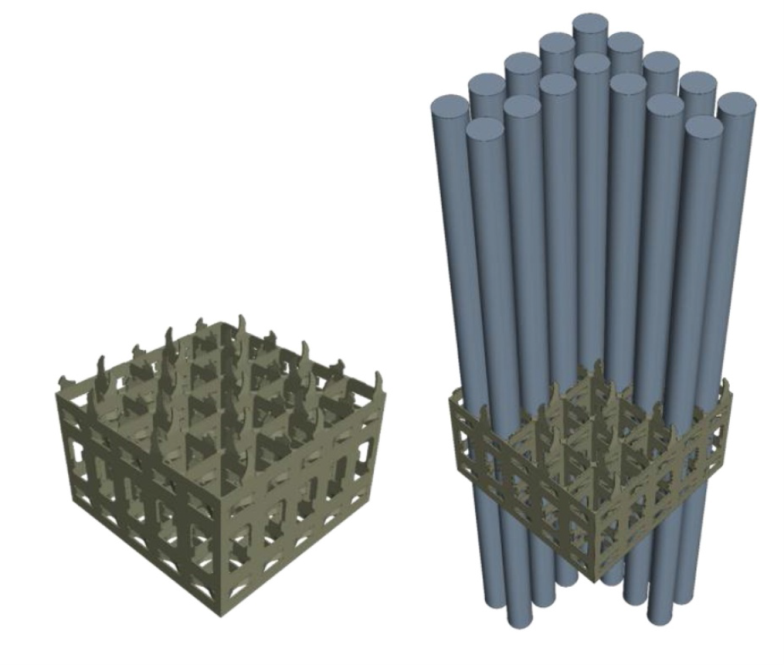
\includegraphics[width=0.5\textwidth]{./figures/3DModel_of_SGMV.png}
\caption{The structure of spacer grid and mixing vanes and a 5x5 fuel rod bundle. }
\label{fig:sgmvcad}
\end{figure}

The development of momentum sources relies on light-weighted test cases with quick turnaround time. As shown in Figure\ref{fig:model2x2}, a 2x2 bundle is created for that purpose, which is the conduit bounded by 9 neighboring fuel pins. The subchannel pitch-to-diameter ratio is 1.33 where the pitch is defined as the distance of two fuel pin centers and the pin diameter is 9.50 mm. The 2x2 bundle has a span of 10 hydraulic diameters. Inflow and outflow conditions are specified for the channel inlet and outflow. Periodic boundary condition is applied to transverse faces while no-slip wall condition applied to all fuel rod surfaces. The computational grid of 2x2 bundle case consists of 59.14 K elements (Figure~\ref{fig:model2x2}). Once the momentum sources are successfully tested in the 2x2 bundle, the next step is to extend the testing geometry to an entire assembly, and eventually to the full core. 

\begin{figure}[!ht]
\centering
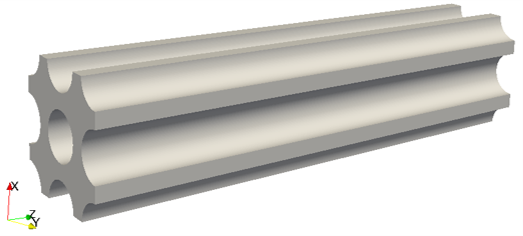
\includegraphics[width=0.5\textwidth]{./figures/3DModel_of_bundle2x2.png}
\caption{A 2x2 subchannel geometry for momentum source development and testing. }
\label{fig:model2x2}
\end{figure}

To drive the flow circulation in a subchannel which has no SGMV, the lateral momentum source terms are devised as follows 
\begin{equation}
  S_x = -\frac{\eta(r)\bullet r sin(\theta)}{\tau_{coupling}}\\
\end{equation}

\begin{equation}
  S_y = \frac{\eta(r)\bullet r cos(\theta)}{\tau_{coupling}}\\
\end{equation}

where the 
$\eta$ is a nominal angular velocity; 
$r$ is the distance from any point to the reference location, that is, the subchannel centerline; 
$\theta$ is the angle between the distance vector and positive x direction and 
$\tau_{coupling}$ is coupling time scale. 
In prototypical fuel rod assembly design, the mixing vanes are deflected in different directions among neighboring subchannels (Figure\ref{fig:sgmvcad}). 
To better reflect that arrangement, each subchannel in the 2x2 bundle test is also given a major axis where the source term in the corresponding direction is enabled (as shown in Figure\ref{fig:sblines}). 
The source terms are accounted as extra acceleration term added back to the body force term in momentum conservation equation to generate the desired flow rotation or pressure drop. 
The macroscale flow movement on the cross-sectional plane is decomposed into two parts: the flow swirling within a specific subchannel and the crossflow among neighboring subchannels. 
A swirling factor ($F_{swirl}$) and a mixing factor ($F_{mix}$) are defined to quantify the swirling and inter-subchannel crossflow, respectively. 
The absolute value of normalized velocity is averaged over the diagonal lines to obtain the swirling factor and over the gap lines to get the mixing factor (Figure~\ref{fig:sblines}).
\begin{equation}
  F_{swirl} = \frac{1}{l}\int\frac{\abs{V_{diag}}}{V_{stream}}dl\\
\end{equation}

\begin{equation}
  F_{mix} = \frac{1}{l}\int\frac{\abs{V_{gap}}}{V_{stream}}dl\\
\end{equation}

\begin{figure}[!ht]
\centering
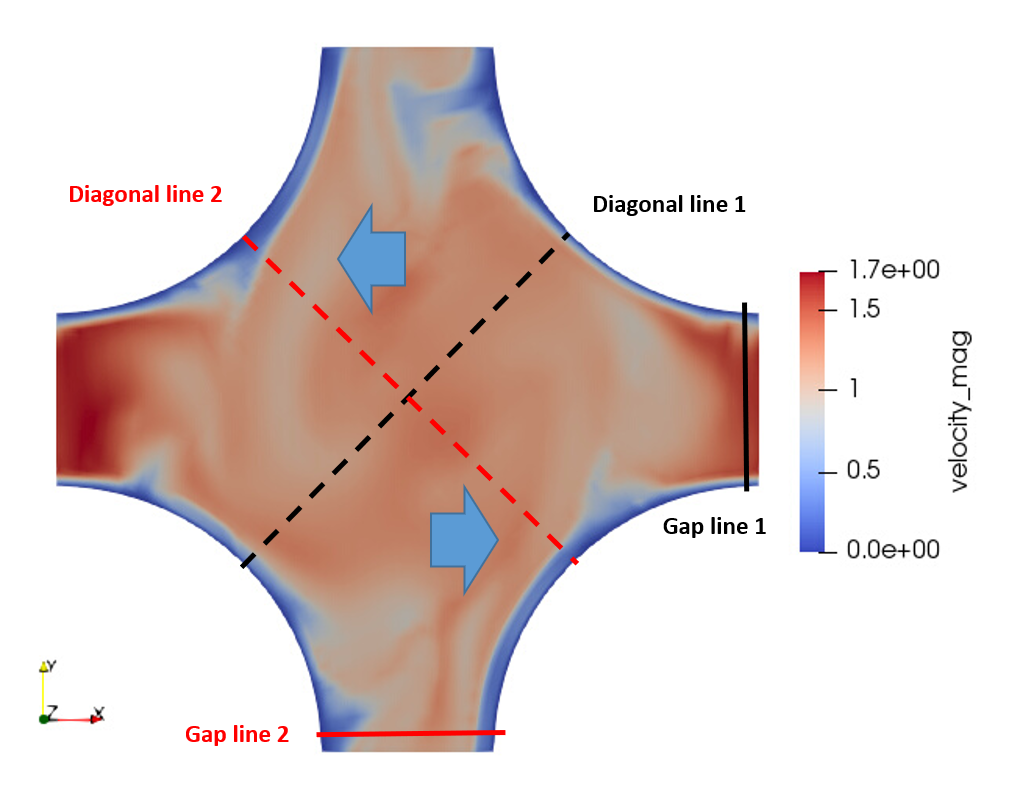
\includegraphics[width=0.5\textwidth]{./figures/Analysis_locations_in_a_subchannel.png}
\caption{The line locations to obtain swirling and mixing factors. Blue arrows indicate the deflection of the simulated mixing vanes. }
\label{fig:sblines}
\end{figure}

The streamwise pressure loss is modeled by adding a momentum source term opposite to the streamwise direction. 

\begin{equation}
  S_z = -\frac{\tau_w \bullet A_{wet}}{V_{channel}}=-\frac{\tau_w \bullet A_{wet}}{A_{wet} \bullet H}=-\frac{\tau_w}{H}\\
\end{equation}

\begin{equation}
  \tau_w = C_fu^2\\
\end{equation}

where $\tau_w$ is the total shear stress caused by the SGMV structures and 
$C_f$ is the effective friction coefficient; 
$A_{wet}$ is the wetted area of channel walls; 
$H$ is the height/distance over which the shear stress is exerted.
Necessary calibration is to be carried out to find out an appropriate friction coefficient that can accurately account for the pressure loss due to SGMV blockage and surface friction.


\subsection{Model Calibration and Verification}
\label{sec:msm3}

The LES of the 5x5 pin bundle were successfully performed and a substantial amount of flow information is collected. 
The instantaneous velocity fields are shown in Figure~\ref{fig:velles}, from which a strong flow mixing is observed caused by the SGMV presence. 
As for all the different LES runs, the cases with higher Reynolds numbers are restarted from the turbulence field fully developed at a lower Reynolds number. 
In other words, the flow solutions obtained at a lower Re serve as the initial condition for the cases at higher Re, which results in significant savings in terms of computing hours. 
Time-averaged first and second order flow quantities are gathered from all cases. 
The subchannel highlighted with a red box is selected for further post-processing. The swirling and mixing factors as well as the pressure drop are extracted from LES flow solutions as the reference to calibrate the corresponding RANS momentum sources

\begin{figure}[!ht]
\centering
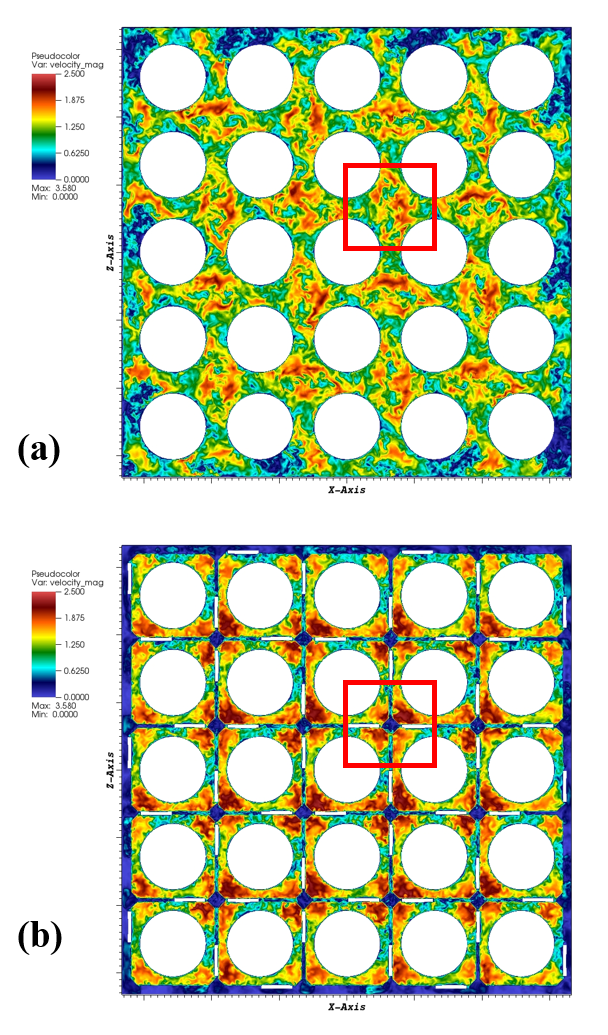
\includegraphics[width=0.5\textwidth]{./figures/LES_solutions_bundle5x5.png}
\caption{The instantaneous velocity fields at (a) a downstream location after SGMV, (b) the onset of mixing vanes region. The subchannel selected for post-processing is highlighted with a red box. }
\label{fig:velles}
\end{figure}

In the meantime, the momentum sources as introduced previously are first implemented in the 2x2 bundle test. 
Interesting results are produced. Note that the test cases are RANS based and thus they would not be able to reproduce a flow field with very fine scale flow fluctuations as shown in Figure~\ref{fig:velles}. 
Rather, the primary research objective here is to reproduce time-averaged macroscale flow characteristics, more specifically, the lateral/cross-sectional flow mixing and the streamwise pressure drop. 
As illustrated in Figure~\ref{fig:streamline}, the momentum sources applied close to the inlet has triggered a streamline pattern shift from a parallel pattern into a swirling pattern.

\begin{figure}[!ht]
\centering
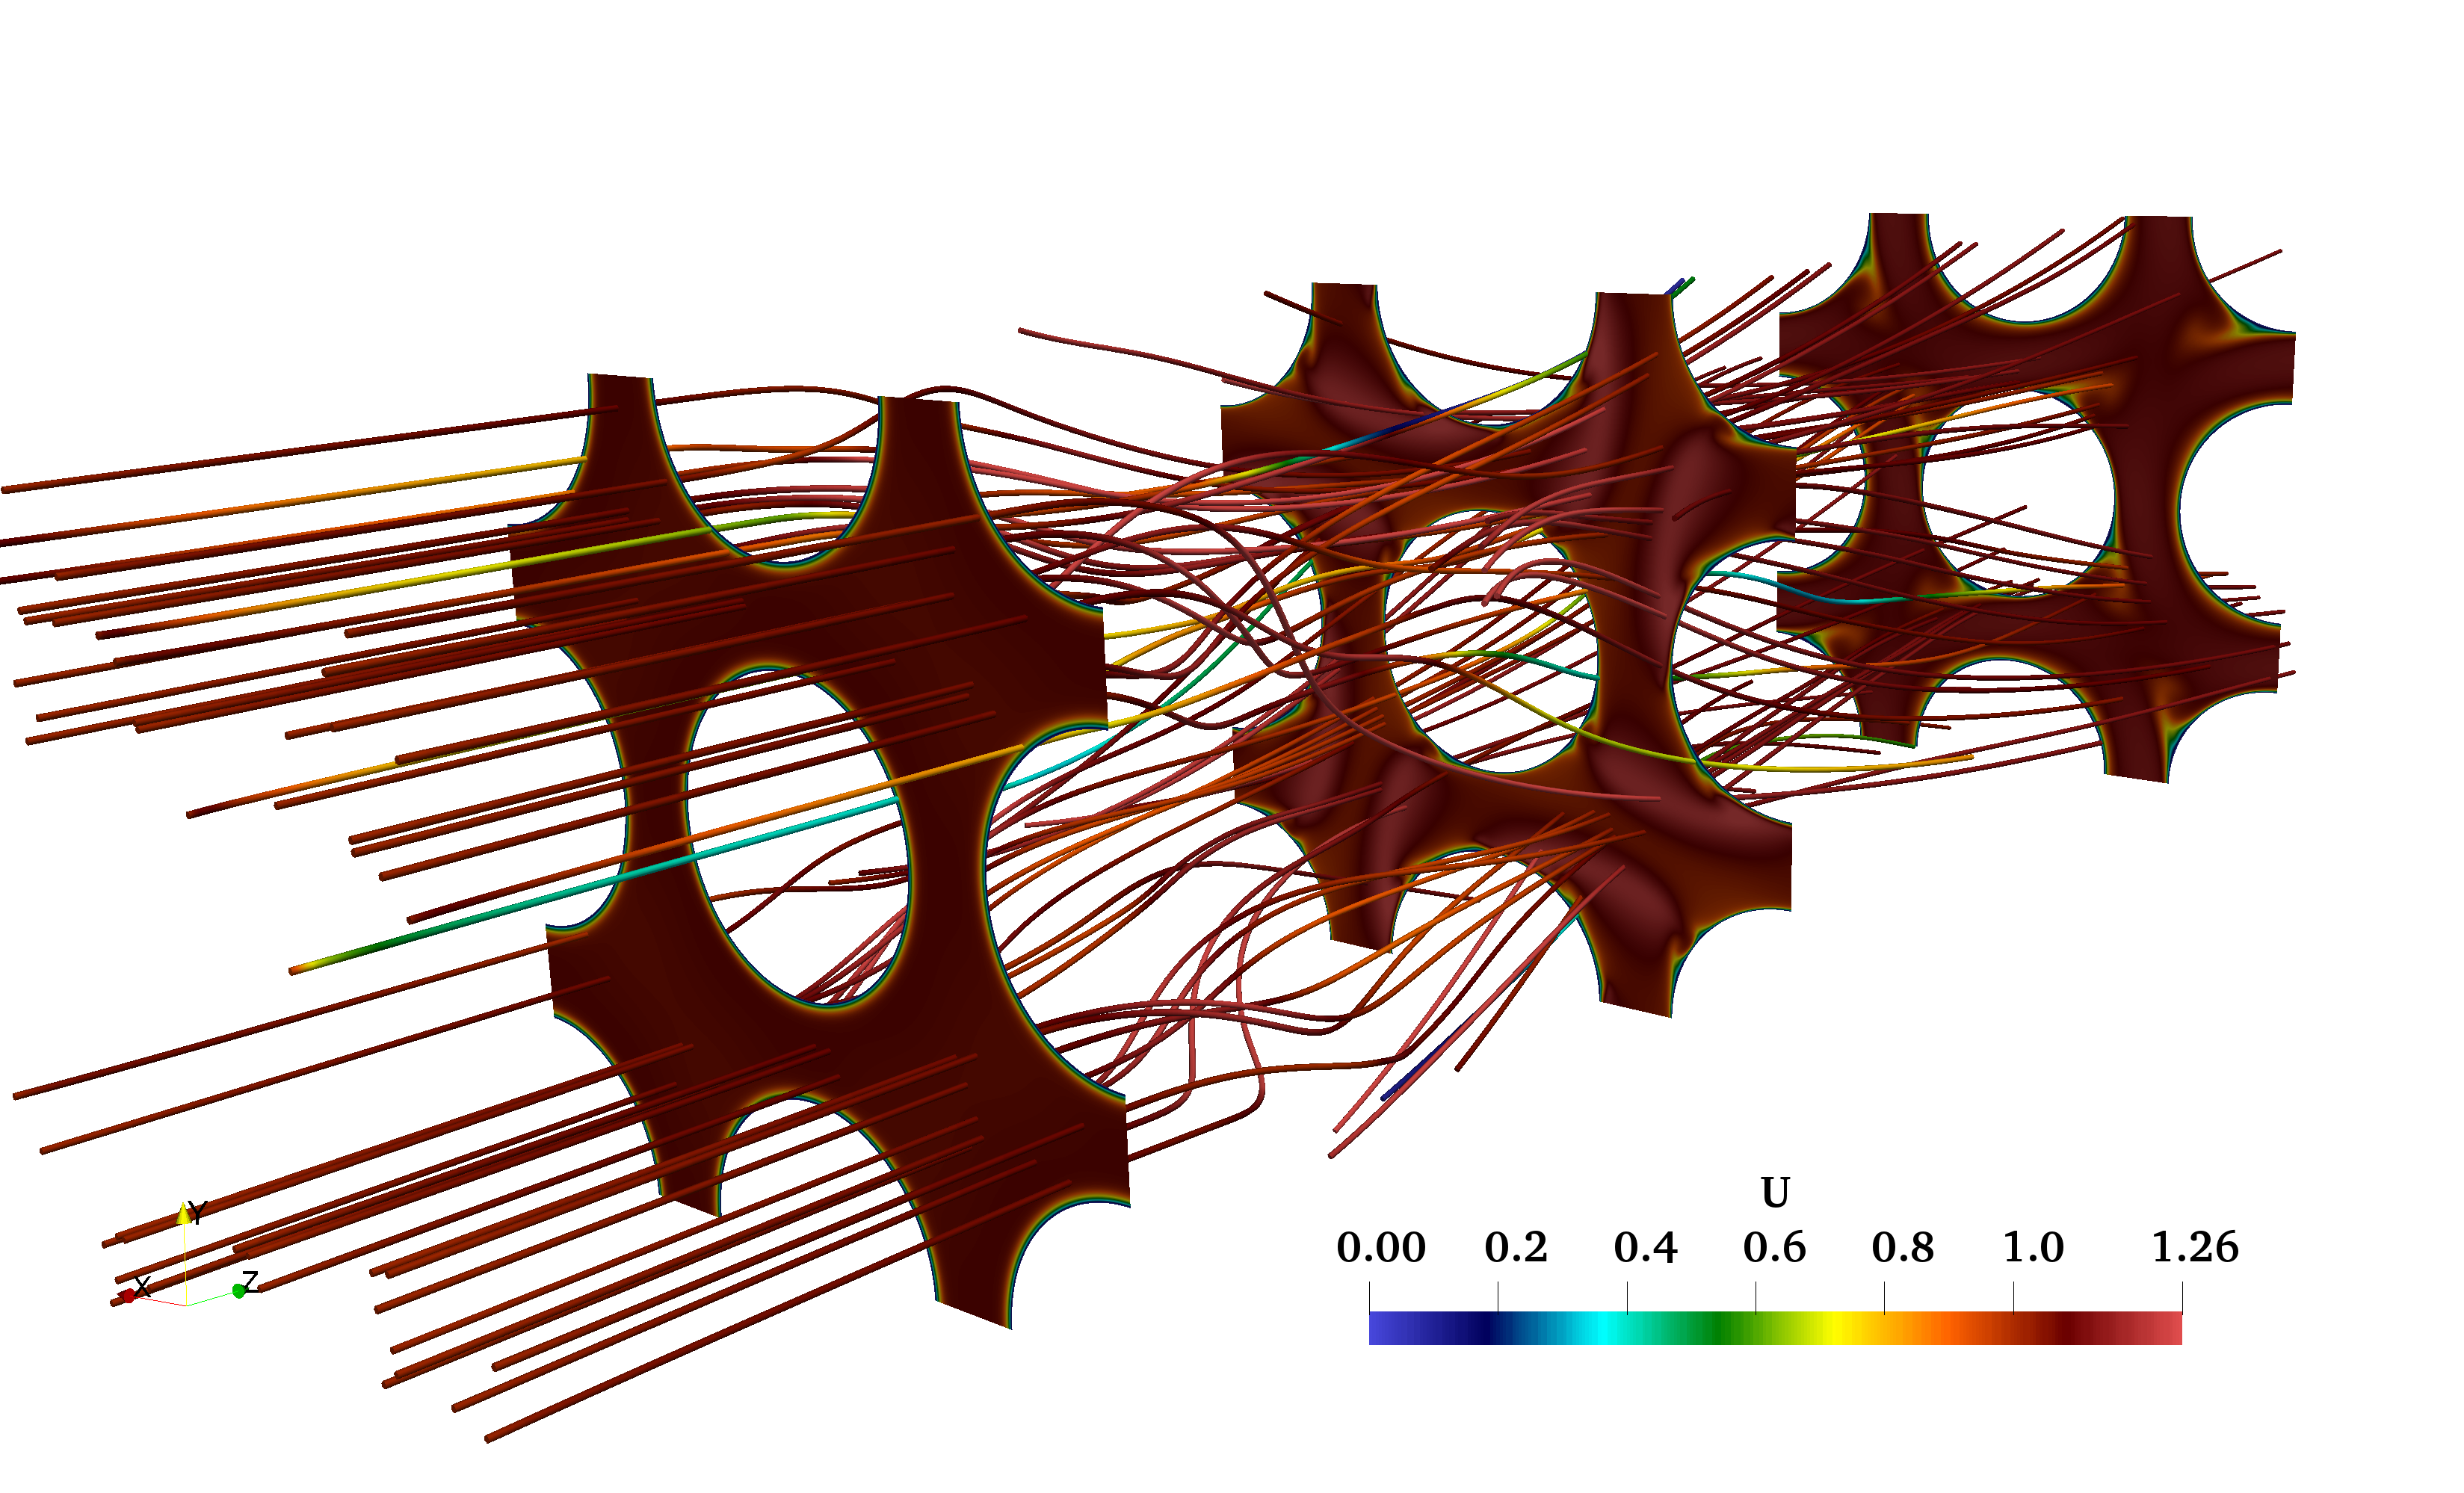
\includegraphics[width=0.5\textwidth]{./figures/RANS_streamlines_bundle2x2.png}
\caption{Streamlines revealing the flow rotation generated by the momentum sources. }
\label{fig:streamline}
\end{figure}

As the two most important figures of merit (FOM) in describing the cross-sectional flow behavior, the swirling and mixing factors are extracted from LES reference solutions. 
The corresponding values serve as an anchor in the calibration of lateral momentum sources dedicated for RANS calculations. 
The comparisons of swirling and mixing factor are presented in Figure~\ref{fig:fswirl} and Figure~\ref{fig:fmix}, respectively. 
It is clearly demonstrated that the RANS momentum sources developed can successfully reproduce the time-averaged macroscale flow physics revealed by the high-fidelity LES reference. 
The momentum sources not only produce the equivalent magnitude of flow swirling and inter-subchannel crossflow, but also capture the consistent decay trend as the flow moves further downstream the mixing vanes. 
As shown in Figure~\ref{fig:fswirl}, due to the mixing vanes deflection, the swirling factors estimated for two perpendicular diagonal lines are noticeably different, and this pattern is well represented by the lateral momentum sources. 
On the other hand, the difference of mixing factors across the two gap lines is relatively smaller. And such a difference is not captured in the RANS calculation and the difference in mixing factor across two perpendicular gap lines is negligible. 
Nevertheless, the RANS mixing factor results are in very good agreement with the averaged value from LES reference. For both the swirling and mixing factors, larger discrepancies are noticed right after the mixing vanes, within 2 hydraulic diameters distance, which indicates room for further improvement of current lateral momentum sources. 

\begin{figure}[!ht]
\centering
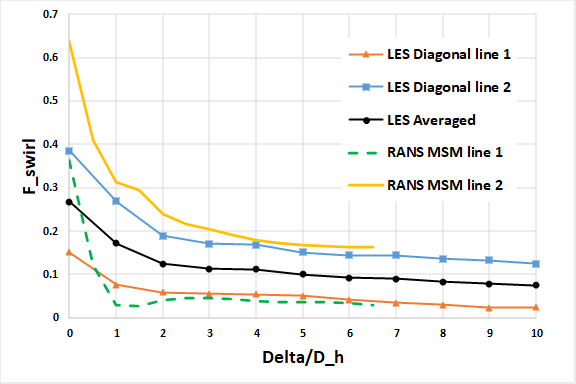
\includegraphics[width=0.5\textwidth]{./figures/Results_swirling_factor.png}
\caption{Comparison of the swirling factors from LES reference and the RANS test with momentum sources at Re = 10,000. }
\label{fig:fswirl}
\end{figure}

\begin{figure}[!ht]
\centering
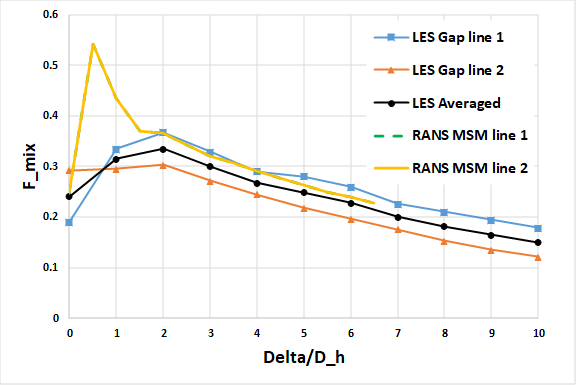
\includegraphics[width=0.5\textwidth]{./figures/Results_mixing_factor.png}
\caption{Comparison of the mixing factors from LES reference and the RANS test with momentum sources at Re = 10,000. }
\label{fig:fmix}
\end{figure}

Besides the swirling and mixing factors, the streamwise pressure loss is another key FOM to quantify the impact of spacer grid and mixing vanes on the coolant flow. Due to the blockage and surface friction, the existence of SGMV would significantly increase the pressure drop, which means a larger pump head will be required to drive the coolant flow. It is also worthwhile to mention that for the incompressible CFD simulations, it is the pressure gradient that dictates the flow physics. As a result, it is intended here to match/reproduce the non-dimensional pressure drop caused by the SGMV rather than the actual pressure value. As shown in Figure~\ref{fig:presloss}, the LES reference solution reports a pressure drop of 1.282 and the RANS test case gives a very similar value of 1.286. Note the here pressure at the end of mixing vanes region ($\Delta/D_h$=0) is set to zero, and the pressure elsewhere is shifted accordingly to preserve the same pressure difference. Similar to what we have noticed in Figure~\ref{fig:fswirl} and Figure~\ref{fig:fmix}, there is some deviation between the RANS results and LES reference within 2~3 hydraulic diameters right after the mixing vanes. The higher pressure observed in LES is attributed to the Bernoulli effect as the cross-sectional area increases when flow exits the SGMV region.  Having said that, the pressure gradient further downstream is well captured, that is, the slope of pressure decrease is close between the RANS (-0.0203) and LES (-0.0184).

\begin{figure}[!ht]
\centering
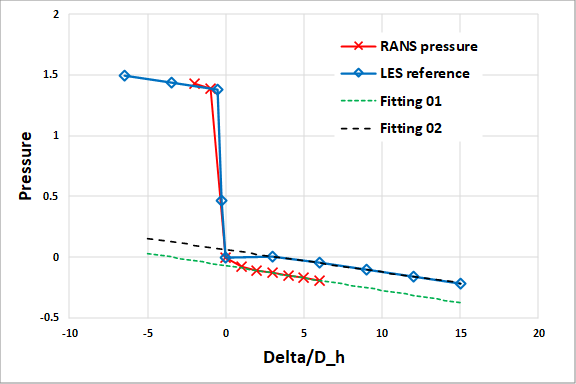
\includegraphics[width=0.5\textwidth]{./figures/Results_pressure_loss.png}
\caption{Comparison of the pressure drop from LES reference and the RANS test with momentum sources at Re = 10,000. }
\label{fig:presloss}
\end{figure}

The calibration has also been carried out for all other Reynolds numbers identified in this investigation, and good agreements are obtained between the LES reference results and the RANS results with momentum sources. More details about the model application in the assembly and full core models will be presented in the following sections. 